\documentclass[paper=a4, fontsize=11pt]{scrartcl} % A4 paper and 11pt font size

\usepackage[T1]{fontenc} % Use 8-bit encoding that has 256 glyphs
\usepackage{fourier} % Use the Adobe Utopia font for the document - comment this line to return to the LaTeX default
\usepackage{amsmath,amsfonts,amsthm, amssymb} % Math packages
\usepackage{multirow}
\usepackage{hyperref}
\usepackage{sectsty} % Allows customizing section commands
\usepackage{graphicx}
\usepackage{tabularx}
\usepackage{enumitem}
\usepackage{wrapfig}
%---------
%CITATIONS
%---------
\usepackage[backend=biber]{biblatex}%TODO: fix to APA
\usepackage{csquotes}
\usepackage[american]{babel} % English language/hyphenation
\DeclareLanguageMapping{american}{american-apa}
\addbibresource{sources.bib}

\usepackage{tikz}
\usepackage{calc}
\def\checkmark{\tikz\fill[scale=0.4] (0,.35) -- (.25,0) -- (1,.7) -- (.25,.15) -- cycle;} 
\def\scalecheck{\resizebox{\widthof{\checkmark}*\ratio{\widthof{x}}{\widthof{\normalsize x}}}{!}{\checkmark}}

\allsectionsfont{\centering \normalfont\scshape} % Make all sections centered, the default font and small caps

\usepackage{fancyhdr} % Custom headers and footers
\pagestyle{fancyplain} % Makes all pages in the document conform to the custom headers and footers
\fancyhead{} % No page header - if you want one, create it in the same way as the footers below
\fancyhead[L]{\tiny{\url{https://github.com/WhereIsJulius/AVC-Code}}}
\fancyhead[R]{\tiny{Jacob Beal\\300378461}}
\fancyfoot[L]{} % Empty left footer
\fancyfoot[C]{} % Empty center footer
\fancyfoot[R]{\thepage} % Page numbering for right footer
\renewcommand{\headrulewidth}{0pt} % Remove header underlines
\renewcommand{\footrulewidth}{0pt} % Remove footer underlines
\setlength{\headheight}{13.6pt} % Customize the height of the header

\numberwithin{equation}{section} % Number equations within sections (i.e. 1.1, 1.2, 2.1, 2.2 instead of 1, 2, 3, 4)
\numberwithin{figure}{section} % Number figures within sections (i.e. 1.1, 1.2, 2.1, 2.2 instead of 1, 2, 3, 4)
%\numberwithin{tabular}{section} % Number tables within sections (i.e. 1.1, 1.2, 2.1, 2.2 instead of 1, 2, 3, 4)

\setlength\parindent{0pt} % Removes all indentation from paragraphs - comment this line for an assignment with lots of text

%----------------------------------------------------------------------------------------
%	TITLE SECTION
%----------------------------------------------------------------------------------------

\newcommand{\horrule}[1]{\rule{\linewidth}{#1}} % Create horizontal rule command with 1 argument of height

\title{
\normalfont\normalsize
\textsc{Victoria University, ENGR101} \\ [25pt] % Your university, school and/or department name(s)
\horrule{0.5pt} \\[0.4cm] % Thin top horizontal rule
\huge AVC Project Report\\ % The assignment title
\horrule{2pt} \\[0.5cm] % Thick bottom horizontal rule
}

\author{Jacob Beal} % Your name

\date{\normalsize\today} % Today's date or a custom date
\begin{document}
\maketitle
\pagebreak
\tableofcontents
\pagebreak

\section{Abstract}
The Following Lab Report details how the application of fundamental engineering
concepts could be used in such a way to construct and operate an Autonomous
Vehicle. This report will detail the design, construction, and programming
decision that we made, the final outcome of the project and the end results,
and in particular issues that arose, and how this was resolved.\\

The Robot in question did not complete the entire maze, and did not complete the
third quadrant.





\section{Introduction}
\subsection{Motivation}
The purpose of the AVC is to demonstrate engineering skills taught in the
ENGR101 Labs; and to work as a team to create an autonomous vehicle. This is
used to solidify the teams understanding of fundamental Engineering concepts.
\subsection{Problem}
%TODO: Fix
The challenge of a self-driving car is not immediately intuitive; the act of %TODO
simply ``following a line''. This involves computing the relative position of
the vehicle compared to the line. The team employed other methods, by tracking
the relative position over time, that will be detailed later in the report.
\subsection{Scope}
The scope of this project was using C/C++, the ENGR101 C Library and skills we
have learned in the Labs for the project. This includes \textit{PID} Error
Correction (Proportional, Integral and Derivative Responses) to follow the 
white line and other techniques taught in lectures.\\
We are also limited by our budget of $V\$100$ for use at the \textit{``part
bazzar''} and the equipment that were provided at the beginning of the
project, the PCB, motors and Raspberry Pi.

\subsection{Motivation}
Understanding how an AVC works and solving a problem is important to the future,
with autonomous vehicles increasing in prevalence, and being developed at break
neck speed, it is of paramount importance that we understand how they work, and
their limitations.








\section{Background}
\subsection{Theory}
\subsubsection{Closed Loops}
A closed loop system is a system which constantly loops, checking a physical
variable. This variable is then computed in such a fashion as to deliver an
output which is used in such a method to influence the physical variable the
next time the loop is checked.\autocite{elfClosedLoops}

A closed loop system is useful in the ``follow the line'' section of the AVC
where a difference in position of the line and the centre of the camera, which
can be used to generate a difference in wheel speed. This difference in wheel
speed can cause a turn in the vehicle

\begin{figure}{h}
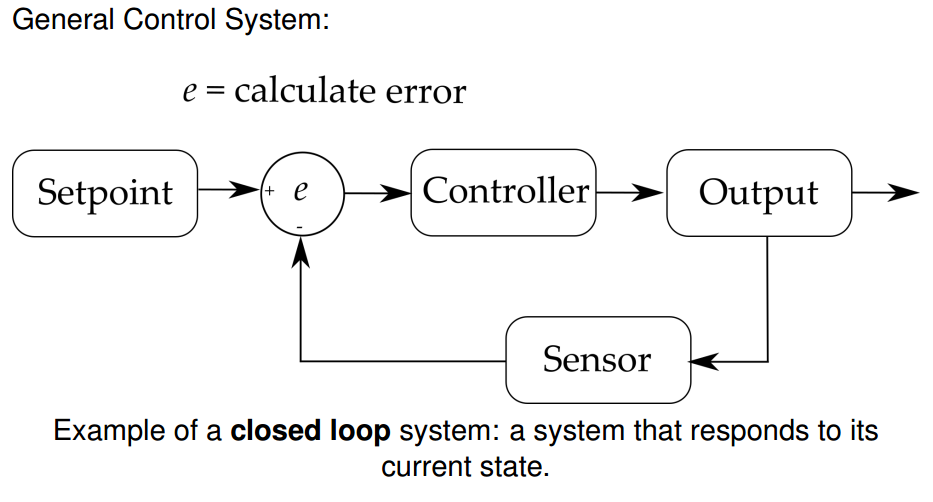
\includegraphics[width=\textwidth]{closedloop}
\centering
\caption{A Closed loop diagram \autocite{elfClosedLoops}}
\end{figure}

\subsubsection{PID}
\textit{PID} stands for \textit{Proportional, Integral and Derivative} response
to a change in the conditions in a closed loop.\\
A proportional response is the current conditions and how it responds to them
immediately.\ i.e.\ the further the object is from the line, the stronger
corrective response is.\\
A integral response checks over time to see whether the car is on one side too
often, and compensates accordingly.\\
A derivative response is related to how quickly the proportional response
changes, and therefore turns the car the other way when it approaches the line.
\begin{figure}[h]
\centering
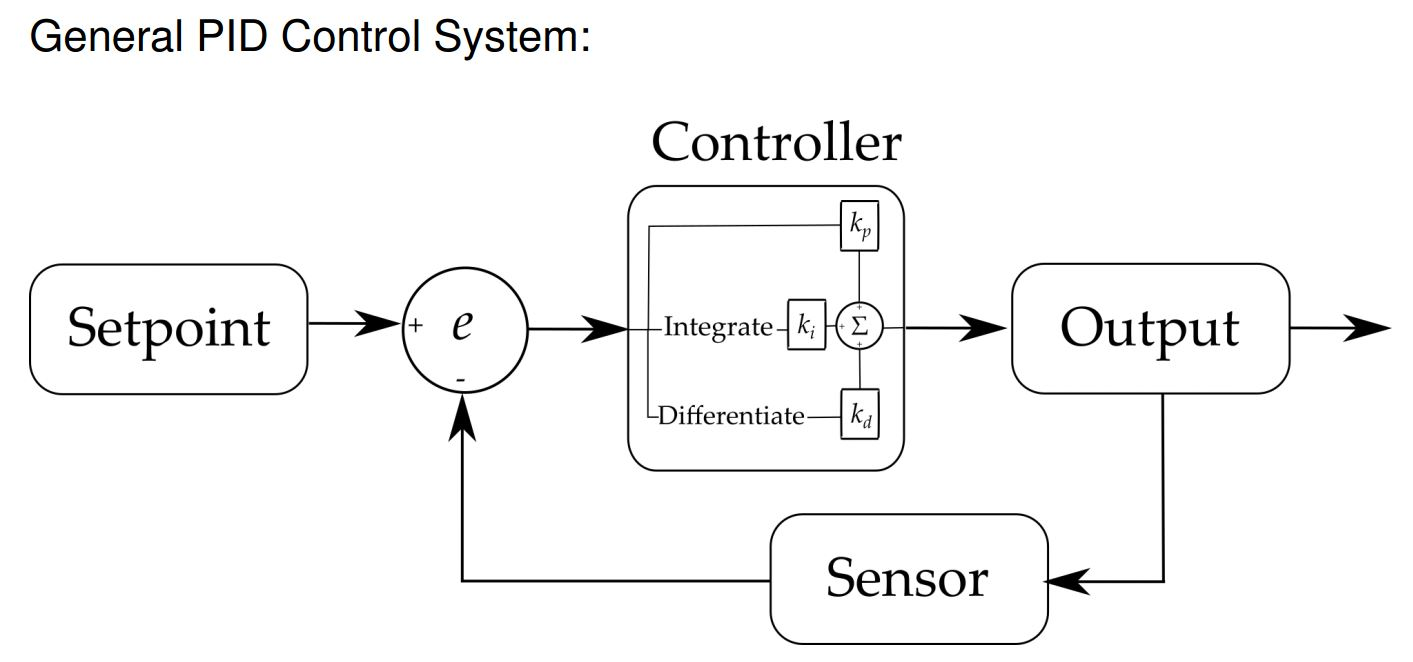
\includegraphics[width=\textwidth]{pid.png}
\caption{A PID system diagram\autocite{elfClosedLoops}}
\end{figure}
\subsubsection{C and Raspberry Pi}
The project will be written using C++, with  an imported C library for the
functionality to control the motors and receive input from sensors.\\
\subsection{Research}
Tuning the PID system should be done in the specific order of Proportional,
Integral then derivative responses. This is because the integral response can
only be turned following the proportional response, so the offset at the end of
the sinusoidal activity, and the derivative response merely acts as a
dampener\autocite{pidTuning}
\autocite{pidVid}
\subsection{The Maze}
\begin{figure}[h]
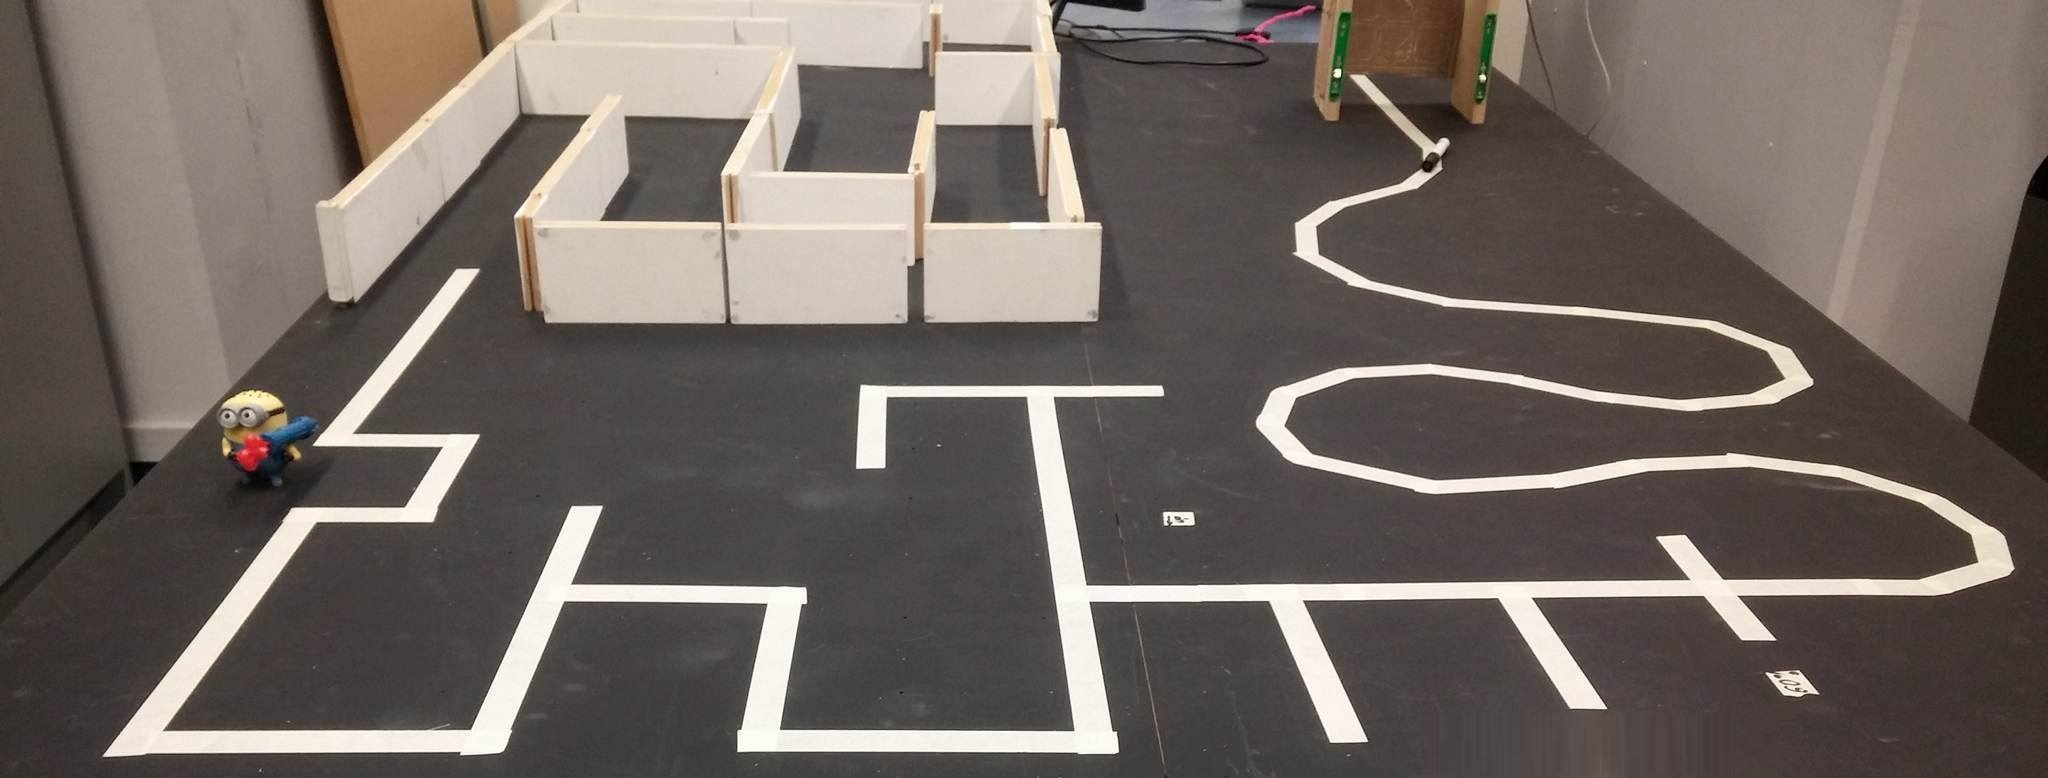
\includegraphics[width=\textwidth]{maze}
\centering
\caption{The Maze used to test the Autonomous vehicle}
\end{figure}



\section{Methods}
\subsection{Equipment}
The AVC Project was based on a Raspberry Pi and the PCB.\\
The Autonomous vehicle was built with a `PiCam' camera (provided), a pair of
motors (provided), a LiFe , 2 `Sharp GP2Y0A41SK0F Analog Distance' sensors, a 3D printed
chassis, and half a ping pong ball.
\subsection{Procedure}
\begin{wrapfigure}{r}{0.5\textwidth}
\begin{center}
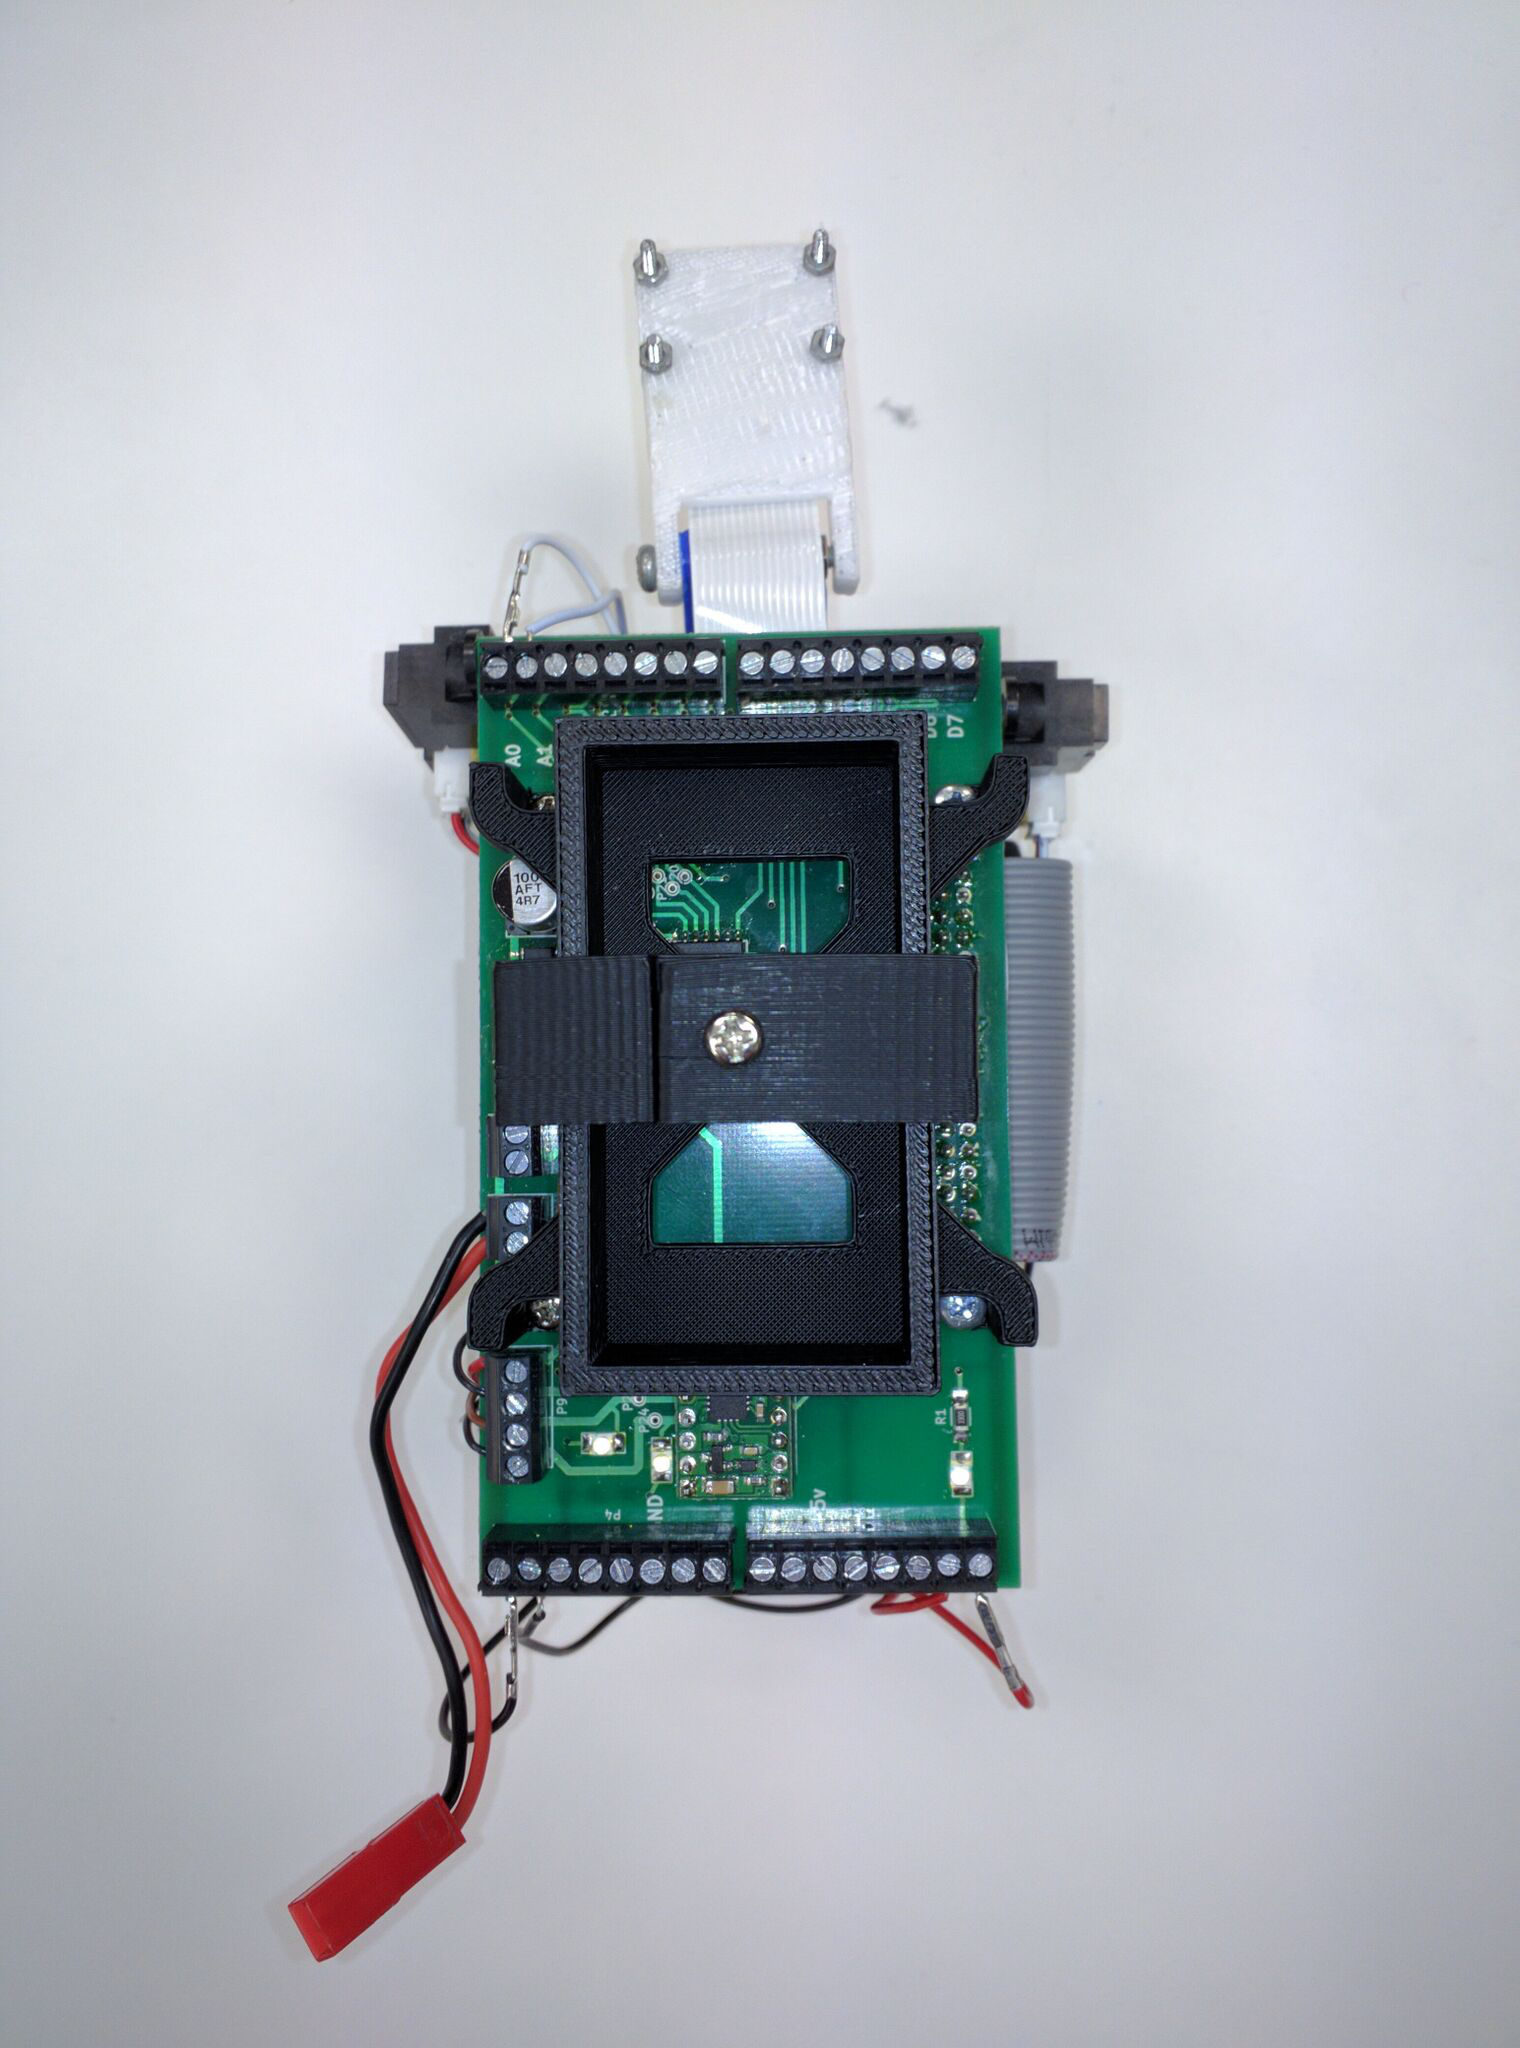
\includegraphics[width=0.3\textwidth]{top-down-view}
\caption{A top-down view of the design chosen for the AVC}
\end{center}
\end{wrapfigure}
\subsubsection{Hardware}
The team first designed the layout of the vehicle. Such that any decisions made
in the code for the vehicle wouldn't have to be rewritten because of hardware
decisions to be made later.\\

The chosen design is primarily based on the initial plastic board and building a
design which would allow both the PCB and the Raspberry Pi, with enough space
left over such that the battery could be safely held without risking damage to
it.\\

As such the design was chosen to hold the battery above the PCB and the
Raspberry Pi, such that it was easy to remove, as it needed to be removed
between testing periods, and on a stable base attached to the PCB, this was
aesthetically appeasing and allowed easy access to the power switch. While also
being smaller than the raised portcullis vertically.\\

\subsubsection{Software}
The network code was first to be created, to deal with the \textit{portcullis}
found in quadrant 1. The code in question sends a predetermined message to the
server using the provided API. The server would return a message which would be
sent in a message to the server, this would cause the portcullis to raise and
allow the vehicle to pass beneath. The code in question can be found in Appendix
2.1.\\%TODO: add link and find the number l8r

The quadrant 2 code works by taking a picture with the `PiCam' and scanning the
vertical middle of the picture taken. The average `whiteness' of the pixels is
found, this was used as a threshold for whether a pixel was `white' or
`black'.\\

The vertical middle pixels were read, and checked against the threshold value to
see if they were `black' or `white'. Using the position of the pixel against the
center. A value of in which direction the `white' pixels were. This value was
multiplied by \verb|CONSTANT_PROPORTIONAL| to find which direction the line was
in.\\

A case was also added in this section for if the entire screen was black, and to
reverse back until the line was found again.


\section{Results}
The vehicle was unable to complete the course and ended half way through the
third quadrant. Upon reaching a terminus of a line, instead of doing a $180\deg$
turn. The vehicle went onto the `correct path'.\\
The \verb|CONSTANT_PROPORTIONAL| was set to $500$. This reflects the fact that
the 

\section{Discussion}
\subsection{Team}
The team had a good general cohesion on the whole, and worked well cooperatively
together during lab sessions. This had a positive effect overall as it led to
better communication of ideas and improved the quality of the vehicle overall.

The lead developer had a general lack of availability due to them
taking \textit{PHYS114}, which consumed alot of their time. This meant that
meetings were less frequent than desired and that bursts of work were
sporadic and more long-winded. Overall this had a negative impact upon the
project as the team had less time and less updates on the progress of individual
aspects of the project.  This led to increased stress in the team, and a slower
development cycle overall. To resolve this in the future more frequent 15 minute
meetings, via a VOIP service, such as google hangouts or skype, would better
keep everyone informed, and allow swifter and more productive use of time\\

The loss of a team member immediately set the team back, and meant that the
amount of time each member had to contribute was greater than other teams. This
decreased team productivity, and led to more stress within the team itself. The
increased workload led to a lower quality of work overall and had a negative
impact upon the project itself. In the future the team needed to better manage
time together to keep development on track.\\

\subsection{Hardware}
The decision to not have a rear wheel and instead have a semi-sphere from a ping
pong ball. This was made because it would give a greater ability to turn the
vehicle and make the AVC more responsive to the change in environment. This was
beneficial in the second quadrant\\

Late into the project the battery clip was redesigned such that the battery was
more securely held without the screw touching the battery, this was so that in
the case of a failure or in the case the vehicle is dropped, the battery would
be largely unaffected and to prevent the Li-Fe battery from leaking.\\

The camera was not correctly plugged in upon initial construction.  As a result
the team fell behind their schedule and was unable to complete the project. 
As a result of this, the PID system that was developed during that period was
ineffective and incorrect as it caused issues that otherwise would not have
existed.\\

\subsection{Software}
The co-efficient of proportionality is much higher then derivative which is
higher than the integral response, to better respond to the present situation.\\
Following a mistake by members of the team in the final weeks, an incorrectly
merged git commit caused the loss of the weeks work, this resulted in the team
being left even further behind then previously. From this the team decided to
only make changes to the code via the github.com UI such that it is always upto
date and so that no merge commits would have to be done\\

Because of time restraints and loss of functioning PID code in the git merge,
the teams took the decision to make a Proportional system as opposed to a PID
one. The constant of proportionality was set to much higher than previously set
and the the speed to be much lower. This would mean that less damping would be
needed (via the differential component of PID) and it freed up development time
to complete the third quadrant.\\

\section{Conclusion}

\section{Bibliography}
\printbibliography

\section{Appendix}

\subsection{Weekly Log}

\subsubsection*{Week 1}
\begin{tabularx}{\textwidth}{clX}
\scalecheck & ALL      & Construct a Project Plan and Contact Julius\\
\scalecheck & Rhaz     & Organise Meeting\\
\scalecheck & Jacob    & Create GitHub and Establish Facebook Chat\\
\scalecheck & Andrew   & Study SSH for Thursday Meeting\\
\scalecheck & Mitchell & Study Unit Testing\\
\scalecheck & Theo     & Make a general plan for the chassis\\
\scalecheck & Julius   & Get in contact with the group
\end{tabularx}

\subsubsection*{Week 2}
\begin{tabularx}{\textwidth}{clX}
\scalecheck  & ALL      & Discuss ideas and start on the AVC Code\\
\scalecheck  & Rhaz     & Keep up to date on weekly tasks\\
& Jacob    & Robot moving in straight line --- appears to work, but haven't tested with a battery yet\\
\scalecheck  & Andrew   & Complete the README.md\\
\scalecheck  & Mitchell & Look into the networking code, and how it works\\
\scalecheck  & Theo     & Figure out how to use the CAD software\\
& Julius   & Show Up --- Not turned up --- Postponed\\
\end{tabularx}

\subsubsection*{Week 3}
\begin{tabularx}{\textwidth}{clX}
\scalecheck & ALL      & Progress update with team members and begin writing progress report\\
\scalecheck & Rhaz     & Robot Opens Gate\\
\scalecheck & Jacob    & Robot Opens Gate\\
\scalecheck & Andrew   & Robot Opens Gate\\
\scalecheck & Mitchell & Update the README create Hardware updates and assist in the hardware efforts.\\
\scalecheck & Theo     & Create a non-powered wheel case and battery case for the robot\\
& Julius   & Show up and contribute to team meetings\\
\end{tabularx}

\subsubsection*{Week 4}
\begin{tabularx}{\textwidth}{clX}
\scalecheck & ALL      & Progress update with team members\\
\scalecheck & Rhaz     & quadrant 1 completed\\
\scalecheck & Jacob    & quadrant 1 completed\\
\scalecheck & Andrew   & quadrant 1 completed\\
\scalecheck & Mitchell & Assist in hardware and pre-reading for quadrant 2\\

& Theo     & Attach sensors to robot so it can detect the maze and obstructions --- postponed as code not up to that section yet.\\
& Julius   & Contribute in some way\\
\end{tabularx}

\subsubsection*{Week 5}
\begin{tabularx}{\textwidth}{clX}
\scalecheck & ALL      & Progress update with team members\\
\scalecheck & Rhaz     & PID system functioning\\
\scalecheck & Jacob    & PID system functioning\\
\scalecheck & Andrew   & PID system functioning\\
\scalecheck & Mitchell & Bug fixing and tinker with PID constants\\
\scalecheck & Theo     & Make battery clip easier\\
& Julius   & Contribute in some way\\
\end{tabularx}

\subsubsection*{Week 6}
\begin{tabularx}{\textwidth}{clX}
& ALL      & quadrant 3 complete\\
& Rhaz     & quadrant 3 complete\\
& Jacob    & quadrant 3 complete\\ 
& Andrew   & quadrant 3 complete\\ 
& Mitchell & quadrant 3 complete\\ 
\scalecheck & Theo     & Attaching sensors to navigate quadrant 4\\
& Julius   & Contribute in some way\\
\end{tabularx}

\subsection{Code Excerpts}

\subsubsection{Networking for Portcullis}
\begin{verbatim}
void network(){
char message[24];							// Assigns memory to password.

connect_to_server("130.195.6.196", 1024);	// Connects to Gate.
send_to_server("Please");					// Requests permission.

receive_from_server(message);				// Assigns the password to 'message'.
send_to_server(message);					// Sends password to server

printf(message);
}
\end{verbatim}

\subsubsection{Straight Line}
\begin{verbatim}
set_motor(1, 100);
set_motor(2, 100);
Sleep(1,0);
set_motor(1, 0);
set_motor(2, 0);
\end{verbatim}

\subsubsection{Average `whiteness' of a picture}
\begin{verbatim}
int determine_average(){
int max = 0;
int min = 255;
int average;

take_picture();							// Takes initial picture.
for(int i = 0; i<320; i++){

if(get_pixel(i, 120, 3)>max){		// Establishes Max.
max = get_pixel(i, 120, 3);
}

if(get_pixel(i, 120, 3)<min){		// Establishes Min.
min = get_pixel(i, 120, 3);

}
}

average = (max+min)/2;
return average;
}
\end{verbatim}
\subsubsection{Finding the white bias and hence direction of travel}
\begin{verbatim}
for(int i=0; i<320; i++){
int error = average_error(i);

if(error >= threshold){				// If RPi sees 'white'
error = 1;						// Converts to binary represenation
seeLine = true;					// The Line can be seen
num_of_white++;
}
else{								// If RPi sees 'black'
error = 0;						// Converts to binary representation
}

current_error = current_error + error*(i-160);
}
\end{verbatim}
Where \verb|average_error| is as follows:\\
\begin{verbatim}
int average_error(int i){
int error1 = get_pixel(i, 116, 3);
int error2 = get_pixel(i, 118, 3);
int error3 = get_pixel(i, 120, 3);
int error4 = get_pixel(i, 122, 3);
int error5 = get_pixel(i, 124, 3);

int average_error = (int) (error5+error4+error3+error2+error1)/5;

return average_error;
}
\end{verbatim}
\end{document}
